\documentclass[10pt,twocolumn,letterpaper]{article}

\usepackage{cvpr}
\usepackage{times}
\usepackage{epsfig}
\usepackage{graphicx}
\usepackage{amsmath}
\usepackage{amssymb}
\usepackage[english]{babel}
\usepackage{blindtext}

% Include other packages here, before hyperref.

% If you comment hyperref and then uncomment it, you should delete
% egpaper.aux before re-running latex.  (Or just hit 'q' on the first latex
% run, let it finish, and you should be clear).
\usepackage[breaklinks=true,bookmarks=false]{hyperref}

\cvprfinalcopy % *** Uncomment this line for the final submission

\def\cvprPaperID{****} % *** Enter the CVPR Paper ID here
\def\httilde{\mbox{\tt\raisebox{-.5ex}{\symbol{126}}}}

% Pages are numbered in submission mode, and unnumbered in camera-ready
%\ifcvprfinal\pagestyle{empty}\fi
\setcounter{page}{4321}
\begin{document}

%%%%%%%%% TITLE
\title{SignNet: Recognize Alphabets in the American Sign Language in Real Time}

\author{
Zeqiang Lai\\
Beijing Institute of Technology\\
{\tt\small laizeqiang@outlook.com}
% For a paper whose authors are all at the same institution,
% omit the following lines up until the closing ``}''.
% Additional authors and addresses can be added with ``\and'',
% just like the second author.
% To save space, use either the email address or home page, not both
\and
Zhiyuan Liang\\
Beijing Institute of Technology\\
{\tt\small secondauthor@i2.org}
\and
Kexiang Huang\\
Beijing Institute of Technology\\
{\tt\small thirdauthor@i2.org}
}

\maketitle
%\thispagestyle{empty}

%%%%%%%%% ABSTRACT
\begin{abstract}
   The ABSTRACT is to be in fully-justified italicized text, at the top
   of the left-hand column, below the author and affiliation
   information. Use the word ``Abstract'' as the title, in 12-point
   Times, boldface type, centered relative to the column, initially
   capitalized. The abstract is to be in 10-point, single-spaced type.
   Leave two blank lines after the Abstract, then begin the main text.
   Look at previous CVPR abstracts to get a feel for style and length.
\end{abstract}

%%%%%%%%% BODY TEXT
\section{Introduction}

\blindtext

\begin{figure}[t]
\begin{center}
 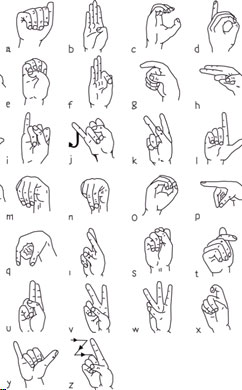
\includegraphics[width=0.8\linewidth]{imgs/NIDCD-ASL-hands-2014.jpg}
\end{center}
\caption{Sign Language Reference}
\label{fig:long}
\end{figure}


\blindtext

%%%%%%%%% Related Work


\section{Related Work}

	
\blindtext

\blindtext



%%%%%%%%% Model Description

\section{SignNet}

As it is mentioned before, we formulate sign language recognition task as a classification problem and we use a modified version of VGG Network \cite{simonyan2014very} to train a classifier for images with different signs. 

In detail, our modifications can be summaried as followed(See figure\ref{fig:arch}). First, we reduce the size of last fully connected network from 4096 to 512. Secondly, we reduce the number of filter of the intermediate convolutional blocks. We make these modifications based on the requirement of live recognition and the assumption that VGG is way to large for the sign language recognition task, which was shown to be correct by the experiment on the ASL Dataset.

\begin{figure*}[ht]
\begin{center}
\fbox{\rule{0pt}{2in} \rule{.9\linewidth}{0pt}}
\end{center}
   \caption{Network architecture}
\label{fig:arch}
\end{figure*}

The exact network architecture can be described in table\ref{table:arch}. The total number of parameter is 10m approximately and the model can achieve 20+fps on an Intel Core I7 CPU.  

\begin{table}[h]
\begin{center}
\begin{tabular}{|l|c|c|c|c|}
\hline
Layer Type & Kernel & Stride & Outputs & Acivation \\
\hline\hline
Conv & 1$\times$3 & 1 & 1$\times$31$\times$3 & ReLU\\
Conv & 1$\times$3 & 1 & 1$\times$31$\times$3 & ReLU\\
Conv & 1$\times$3 & 1 & 1$\times$31$\times$3 & ReLU\\
Conv & 1$\times$3 & 1 & 1$\times$31$\times$3 & ReLU\\
Conv & 1$\times$3 & 1 & 1$\times$31$\times$3 & ReLU\\
FC & 1$\times$3 & 1 & 1$\times$31$\times$3 & ReLU\\
\hline
\end{tabular}
\end{center}
\caption{Results.  Ours is better.}
\label{table:arch}
\end{table}


%%%%%%%%% Experiments

\section{Vanilla Experiments}

In this section, we introduce the experiments we have conducted using the model described in the previous section.

\subsection{ASL Dataset}

ASL Alphabet\cite{noauthor_asl_nodate} is a collection of images of alphabets from the American Sign Language, which is public available on Kaggle. The training data set contains 87,000 images which are 200$\times$200 pixels. There are 29 classes, of which 26 are for the letters A-Z and 3 classes for SPACE, DELETE and NOTHING. The test data set contains a mere 29 images, which is too small for an effective test.

For testing, we use another dataset - ASL Alphabet Test\cite{noauthor_asl_nodate-1}. This dataset is collected by a different person and it consists of 870 images with various background. There are 30 images for each symbol, A-Z, delete, space, and nothing and every image is 200$\times$200 8-bit photo, which is the same as it is in ASL Alphabet. 

\subsection{Training Detail}

We train our model with cross entropy loss. We adopt Adam optimizer\cite{kingma2014adam} with default parameters. The learning rate is set to 0.0001 for the first epoch, and decayed by 0.7 every other epoch. 

During training, we randomly flip images horizontally. After that, the images are converted into grayscale and resized to 64$\times$64 to reduce computational complexity. 

\subsection{Results}

The training and testing result is shown in table\ref{table:result}

\begin{table}[h]
\begin{center}
\begin{tabular}{|l|c|}
\hline
Dataset & Accuuracy \\
\hline\hline
Theirs & Frumpy \\
Yours & Frobbly \\
Ours & Makes one's heart Frob\\
\hline
\end{tabular}
\end{center}
\caption{Results.   Ours is better.}
\label{table:result}
\end{table}

\section{Improvement}

The ASL Alphabet dataset has small background variations and it is hard to train a model that works well in real environment, which is shown in the experiments mentioned in the previous section.

As a result, we decided to make a dataset on our own. In order to reduce the negative effect of background on prediction, we use background subtraction technique to remove it while recording dataset, and we use the same method to remove background in testing and inference stages. In this way, we can basically obtain a model that is able to work under limited environment.

\subsection{Custom Dataset}

Instead of collecting more data with different backgrounds, we choose to make a dataset without background directly, because recording dataset with diverse backgrounds is time-consuming and laborious.

In summary, we record a dataset that consists of xx hours video. The dataset is publicly available on Github.

\subsection{Background Subtraction}

We choose Running Average Background Subtraction algorithm to detect and remove background, because it is fast and easy to implement.

The key idea of this algorithm is to compute a reference background image using running average of first few frames in a video, and subtract the current image with respect to the reference background, and finally compare it with  to the certain threshold. Pixels that exceed threshold are considered to be foreground, while all the others are background.
 
 After comparison, we could get a background mask. Instead of using binary mask directly, we use the mask to remove background to get a grayscale hand image, because some signs require counting fingers to be recognized correctly. See figure. 
 
 \begin{figure}[h]
\begin{center}
\fbox{\rule{0pt}{2in} \rule{0.9\linewidth}{0pt}}
   %\includegraphics[width=0.8\linewidth]{egfigure.eps}
\end{center}
   \caption{Origin, mask and grayscale hand images}
\label{fig:long}
\label{fig:onecol}
\end{figure}


\subsection{Experiment}

\blindtext

\begin{figure}[h]
\begin{center}
\fbox{\rule{0pt}{2in} \rule{0.9\linewidth}{0pt}}
   %\includegraphics[width=0.8\linewidth]{egfigure.eps}
\end{center}
   \caption{Confusion matrix}
\label{fig:long}
\label{fig:onecol}
\end{figure}



%%%%%%%%% Conclusion

\section{Conclusion}
\blindtext

{\small
\bibliographystyle{ieee_fullname}
\bibliography{egbib}
}

\end{document}
